\documentclass{beamer}
\usepackage[utf8]{inputenc}

\usetheme{Madrid}
\usecolortheme{default}
\usepackage{amsmath,amssymb,amsfonts,amsthm}
\usepackage{txfonts}
\usepackage{tkz-euclide}
\usepackage{listings}
\usepackage{adjustbox}
\usepackage{array}
\usepackage{tabularx}
\usepackage{gvv}
\usepackage{lmodern}
\usepackage{circuitikz}
\usepackage{tikz}
\usepackage{graphicx}

\setbeamertemplate{page number in head/foot}[totalframenumber]

\usepackage{tcolorbox}
\tcbuselibrary{minted,breakable,xparse,skins}

\definecolor{bg}{gray}{0.95}
\DeclareTCBListing{mintedbox}{O{}m!O{}}{%
breakable=true,
listing engine=minted,
listing only,
minted language=#2,
minted style=default,
minted options={%
linenos,
gobble=0,
breaklines=true,
breakafter=,,
fontsize=\small,
numbersep=8pt,
#1},
boxsep=0pt,
left skip=0pt,
right skip=0pt,
left=25pt,
right=0pt,
top=3pt,
bottom=3pt,
arc=5pt,
leftrule=0pt,
rightrule=0pt,
bottomrule=2pt,
toprule=2pt,
colback=bg,
colframe=orange!70,
enhanced,
overlay={%
\begin{tcbclipinterior}
\fill[orange!20!white] (frame.south west) rectangle ([xshift=20pt]frame.north west);
\end{tcbclipinterior}},
#3,
}
\lstset{
language=C,
basicstyle=\ttfamily\small,
keywordstyle=\color{blue},
stringstyle=\color{orange},
commentstyle=\color{green!60!black},
numbers=left,
numberstyle=\tiny\color{gray},
breaklines=true,
showstringspaces=false,
}

\title{8.2.7}
\date{October 5 , 2025}
\author{EE25BTECH11043 - Nishid Khandagre}

\begin{document}

\frame{\titlepage}

\begin{frame}{Question}
Find the coordinates of the focus, vertex, eccentricity, axis of the conic section, the equation of the directrix and the length of the latus rectum. \\
$16x^2 + y^2 = 16$
\end{frame}

\begin{frame}{Theoretical Solution}
We use an affine transformation to convert the conic equation to its standard form.
\begin{align}
    \vec{x}^\top\vec{V}\vec{x} + 2\vec{u}^\top\vec{x} + f = 0
\end{align}
The symmetric matrix $\vec{V}$ is spectrally decomposed to align axes with eigenvectors.
\begin{align}
    \vec{V} = \vec{P}\vec{D}\vec{P}^\top, \text{ } \vec{D} = \myvec{\lambda_1 & 0 \\ 0 & \lambda_2}, \text{ } \vec{P}^\top\vec{P} = \vec{I}
\end{align}
\end{frame}

\begin{frame}{Theoretical Solution}
Substituting the decomposition into the conic equation.
\begin{align}
    \vec{x}^\top\vec{P}\vec{D}\vec{P}^\top\vec{x} + 2\vec{u}^\top\vec{x} + f = 0
\end{align}
A rotation
\begin{align}
    \vec{x_r} = \vec{P}^\top\vec{x} 
\end{align}
aligns the conic with the coordinate axes.
\begin{align}
    \vec{x} = \vec{P}\vec{x_r}
\end{align}
\end{frame}

\begin{frame}{Theoretical Solution}
Applying the rotation to the conic equation.
\begin{align}
    \brak{\vec{P}\vec{x_r}}^\top\vec{P}\vec{D}\vec{P}^\top\brak{\vec{P}\vec{x_r}} + 2\vec{u}^\top\brak{\vec{P}\vec{x_r}} + f &= 0 \\
    \vec{x_r}^\top\vec{P}^\top\vec{P}\vec{D}\vec{P}^\top\vec{P}\vec{x_r} + 2\brak{\vec{P}^\top\vec{u}}^\top\vec{x_r} + f &= 0 \\
    \vec{x_r}^\top\vec{D}\vec{x_r} + 2\vec{u_r}^\top\vec{x_r} + f &= 0
\end{align}
\end{frame}

\begin{frame}{Theoretical Solution}
A translation 
\begin{align}
    \vec{x_c} = \vec{x_r} + \vec{D}^{-1}\vec{u_r}
\end{align}
moves the conic's center to the origin.
\begin{align}
    f_c = f - \vec{u_r}^\top\vec{D}^{-1}\vec{u_r}
\end{align}
The center of the conic in the original coordinates is 
\begin{align}
    \vec{c} = -\vec{V}^{-1}\vec{u}
\end{align}
\begin{align}
    \vec{c} = -\brak{\vec{P}\vec{D}\vec{P}^\top}^{-1}\vec{u} = -\vec{P}\vec{D}^{-1}\vec{P}^\top\vec{u} = -\vec{P}\vec{D}^{-1}\vec{u_r}
\end{align}
\end{frame}

\begin{frame}{Theoretical Solution}
The complete transformation from original to centered coordinates is 
\begin{align}
    \vec{x_c} = \vec{P}^\top\brak{\vec{x}-\vec{c}}
\end{align}
\begin{align}
    \vec{x_c} &= \vec{P}^\top\vec{x} + \vec{D}^{-1}\vec{u_r} = \vec{P}^\top\vec{x} - \vec{P}^\top\vec{c} = \vec{P}^\top\brak{\vec{x}-\vec{c}} \\
    \implies \vec{x} &= \vec{P}\vec{x_c} + \vec{c} \label{eq:71}
\end{align}
\end{frame}

\begin{frame}{Theoretical Solution}
The given conic equation
\begin{align}
    16x^2 + y^2 &= 16 \\
    \frac{16x^2}{16} + \frac{y^2}{16} &= \frac{16}{16} \\
    \frac{x^2}{1} + \frac{y^2}{16} &= 1
\end{align}
This is an ellipse centered at (0,0) with major axis along the y-axis.
\begin{align}
    \vec{V} = \myvec{1 & 0 \\ 0 & \frac{1}{16}}, \text{ } \vec{u} = \myvec{0 \\ 0}, \text{ } f = -1
\end{align}
\end{frame}

\begin{frame}{Theoretical Solution}
The major axis corresponds to smaller eigenvalue.
\begin{align}
    \lambda_1 = \frac{1}{16}, \text{ } \lambda_2 = 1, \text{ } \vec{P} = \myvec{0 & 1 \\ 1 & 0}, \text{ } \vec{c} = \myvec{0 \\ 0}
\end{align}
Applying the rotation to find the canonical coordinates.
\begin{align}
    \vec{x_c} = \vec{P}^\top\vec{x} \implies \myvec{x_c \\ y_c} = \myvec{0 & 1 \\ 1 & 0}\myvec{x \\ y} = \myvec{y \\ x}
\end{align}
\end{frame}

\begin{frame}{Theoretical Solution}
The standard form of the ellipse in canonical coordinates.
\begin{align}
    \frac{x_c^2}{-f/\lambda_1} + \frac{y_c^2}{-f/\lambda_2} = 1
\end{align}
From this, $a^2 = -f/\lambda_1 = -(-1)/(1/16) = 16 \implies a=4$ (major semi-axis) and $b^2 = -f/\lambda_2 = -(-1)/1 = 1 \implies b=1$ (minor semi-axis).
\end{frame}

\begin{frame}{Theoretical Solution}
Now we can calculate the properties:
\begin{align}
    e &= \sqrt{1 - \frac{b^2}{a^2}} = \sqrt{1 - \frac{1}{16}} = \frac{\sqrt{15}}{4} \\
    \vec{f_c} &= \pm ae \vec{e_1} \text{ (if major axis is x-axis)} \\
    &= \pm \sqrt{a^2-b^2} \vec{e_1} = \pm \sqrt{16-1} \vec{e_1} = \pm\sqrt{15}\vec{e_1} \text{ (along canonical y-axis)} \\
    \vec{v_c} &= \pm a\vec{e_1} = \pm 4\vec{e_1} \text{ (along canonical y-axis)} \\
    \vec{d_c} &: \vec{e_1}^\top\vec{x_c} = \pm \frac{a}{e} = \pm \frac{4}{\sqrt{15}/4} = \pm\frac{16}{\sqrt{15}} \\
    L &= \frac{2b^2}{a} = \frac{2(1)^2}{4} = \frac{1}{2}
\end{align}
\end{frame}

\begin{frame}{Theoretical Solution}
Transforming properties back to the original coordinate system using \eqref{eq:71}.
\begin{align}
    \vec{f} &= \vec{P}\brak{\pm \sqrt{15}\vec{e_1}} = \pm \sqrt{15}\vec{e_2} = \myvec{0 \\ \pm \sqrt{15}} \\
    \vec{v} &= \vec{P}\brak{\pm 4\vec{e_1}} = \pm 4\vec{e_2} = \myvec{0 \\ \pm 4} \\
    \vec{d} &: \vec{e_2}^\top\vec{x} = \pm \frac{16}{\sqrt{15}} \implies \myvec{0 & 1}\vec{x} = \pm \frac{16}{\sqrt{15}}
\end{align}
\end{frame}

\begin{frame}{Theoretical Solution Summary}
\begin{center}
\begin{tabular}{|l|c|}
    \hline
    \textbf{Property} & \textbf{Value} \\
    \hline
    Eccentricity & $\frac{\sqrt{15}}{4}$ \\
    \hline
    Axis & $x=0$ (Y-axis, major axis) \\
    \hline
    Vertices & $\brak{0, \pm 4}$ \\
    \hline
    Foci & $\brak{0, \pm \sqrt{15}}$ \\
    \hline
    Directrices & $y = \pm \frac{16}{\sqrt{15}}$ \\
    \hline
    Latus Rectum & $\frac{1}{2}$ \\
    \hline
\end{tabular}
\end{center}
\end{frame}

\begin{frame}[fragile]
\frametitle{C Code}
\begin{lstlisting}{c}
#include <math.h>

// Function to calculate ellipse properties and pass them back via pointers
void calculateEllipseProperties(
    double a_val,
    double b_val,
    double* focus_y_ptr,
    double* vertex_y_ptr,
    double* eccentricity_ptr,
    double* directrix_y_ptr,
    double* latus_rectum_ptr
) {
\end{lstlisting}
\end{frame}

\begin{frame}[fragile]
\frametitle{C Code}
\begin{lstlisting}{c}
    double c_val = sqrt(a_val * a_val - b_val * b_val);

    *focus_y_ptr = c_val;
    *vertex_y_ptr = a_val;
    *eccentricity_ptr = c_val / a_val;
    *directrix_y_ptr = a_val / (*eccentricity_ptr); // Use the calculated eccentricity
    *latus_rectum_ptr = (2 * b_val * b_val) / a_val;
}
\end{lstlisting}
\end{frame}

\begin{frame}[fragile]
\frametitle{Python Code (using C shared output)}
\begin{lstlisting}{python}
import ctypes
import numpy as np
import matplotlib.pyplot as plt

# Load the shared library
lib_conic = ctypes.CDLL("./code14.so") 

# Define the argument types and return type for the C function
lib_conic.calculateEllipseProperties.argtypes = [
    ctypes.c_double,  # a_val
    ctypes.c_double,  # b_val
    ctypes.POINTER(ctypes.c_double), # focus_y_ptr
    ctypes.POINTER(ctypes.c_double), # vertex_y_ptr
    ctypes.POINTER(ctypes.c_double), # eccentricity_ptr
    ctypes.POINTER(ctypes.c_double), # directrix_y_ptr
    ctypes.POINTER(ctypes.c_double)  # latus_rectum_ptr
]
lib_conic.calculateEllipseProperties.restype = None
\end{lstlisting}
\end{frame}

\begin{frame}[fragile]
\frametitle{Python Code (using C shared output)}
\begin{lstlisting}{python}
# --- Analyze the Ellipse: 16x^2 + y^2 = 16 ---
# From 16x^2 + y^2 = 16, divide by 16: x^2/1 + y^2/16 = 1
# This is an ellipse centered at (0,0) with major axis along y.
# a^2 = 16 => a = 4 (major semi-axis)
# b^2 = 1 => b = 1 (minor semi-axis)
a_val = 4.0
b_val = 1.0
center = np.array([0.0, 0.0]) # Center is (0,0)

# Create ctypes doubles to hold the results from the C function
focus_y_result = ctypes.c_double()
vertex_y_result = ctypes.c_double()
eccentricity_result = ctypes.c_double()
directrix_y_result = ctypes.c_double()
latus_rectum_result = ctypes.c_double()
\end{lstlisting}
\end{frame}

\begin{frame}[fragile]
\frametitle{Python Code (using C shared output)}
\begin{lstlisting}{python}
# Call the C function to get the ellipse properties
lib_conic.calculateEllipseProperties(
    a_val, b_val,
    ctypes.byref(focus_y_result),
    ctypes.byref(vertex_y_result),
    ctypes.byref(eccentricity_result),
    ctypes.byref(directrix_y_result),
    ctypes.byref(latus_rectum_result)
)

# Extract the values from the ctypes doubles
focus_y = focus_y_result.value
vertex_y = vertex_y_result.value
eccentricity = eccentricity_result.value
directrix_y = directrix_y_result.value
latus_rectum = latus_rectum_result.value
\end{lstlisting}
\end{frame}

\begin{frame}[fragile]
\frametitle{Python Code (using C shared output)}
\begin{lstlisting}{python}
# Calculate the other points needed for plotting and printing
# Vertices (along major axis, y-axis)
vertex1 = np.array([0.0, vertex_y])
vertex2 = np.array([0.0, -vertex_y])

# Foci (along major axis, y-axis)
focus1 = np.array([0.0, focus_y])
focus2 = np.array([0.0, -focus_y])

print(f"--- Conic Section Properties (Ellipse: 16x^2 + y^2 = 16) ---")
print(f"Center: ({center[0]:.0f}, {center[1]:.0f})")
print(f"Vertices: ({vertex1[0]:.0f}, {vertex1[1]:.0f}) and ({vertex2[0]:.0f}, {vertex2[1]:.0f})")
print(f"Foci: ({focus1[0]:.2f}, {focus1[1]:.2f}) and ({focus2[0]:.2f}, {focus2[1]:.2f})")
print(f"Eccentricity: {eccentricity:.4f}")
\end{lstlisting}
\end{frame}

\begin{frame}[fragile]
\frametitle{Python Code (using C shared output)}
\begin{lstlisting}{python}
print(f"Axis of the conic section: y-axis (x=0) is the major axis")
print(f"Equation of Directrices: y = {directrix_y:.2f} and y = {-directrix_y:.2f}")
print(f"Length of Latus Rectum: {latus_rectum:.2f}")

# --- Plotting the Ellipse with improved aesthetics ---
plt.figure(figsize=(10, 10))
ax = plt.gca()

# Generate points for the ellipse
theta = np.linspace(0, 2 * np.pi, 200)
x_ellipse = b_val * np.cos(theta)
y_ellipse = a_val * np.sin(theta)
plt.plot(x_ellipse, y_ellipse, "blue", linewidth=2, label='Ellipse $16x^2 + y^2 = 16$')
\end{lstlisting}
\end{frame}

\begin{frame}[fragile]
\frametitle{Python Code (using C shared output)}
\begin{lstlisting}{python}
# Plot Center (Black dot)
plt.scatter(0, 0, color='black', s=30, zorder=5, label='Center (0,0)')

# Plot Vertices (Red dots)
plt.scatter(0, vertex_y, color='red', s=30, zorder=5, label=f'Vertices (0, $\\pm${vertex_y:.0f})')
plt.scatter(0, -vertex_y, color='red', s=30, zorder=5)
# Annotations for vertices
plt.annotate(f'(0, {vertex_y:.0f})', (0, vertex_y), textcoords="offset points", xytext=(5, 5), ha='left', color='red', fontsize=10)
plt.annotate(f'(0, {-vertex_y:.0f})', (0, -vertex_y), textcoords="offset points", xytext=(5, 5), ha='left', color='red', fontsize=10)
\end{lstlisting}
\end{frame}

\begin{frame}[fragile]
\frametitle{Python Code (using C shared output)}
\begin{lstlisting}{python}
# Plot Foci (Green dots)
plt.scatter(0, focus_y, color='green', s=30, zorder=5, label=f'Foci (0, $\\pm${focus_y:.2f})')
plt.scatter(0, -focus_y, color='green', s=30, zorder=5)
plt.annotate(f'(0, {focus_y:.2f})', (0, focus_y), textcoords="offset points", xytext=(5, -15), ha='left', color='green', fontsize=10)
plt.annotate(f'(0, {-focus_y:.2f})', (0, -focus_y), textcoords="offset points", xytext=(5, 5), ha='left', color='green', fontsize=10)
# Plot Directrices (Magenta dashed lines)
x_plot_limits = np.array([-b_val * 2.5, b_val * 2.5]) # Set x limits for directrix lines
plt.plot(x_plot_limits, [directrix_y, directrix_y], 'b--', linewidth=1.5, label=f'Directrices y = $\\pm${directrix_y:.2f}')
plt.plot(x_plot_limits, [-directrix_y, -directrix_y], 'b--', linewidth=1.5)
\end{lstlisting}
\end{frame}

\begin{frame}[fragile]
\frametitle{Python Code (using C shared output)}
\begin{lstlisting}{python}
# Plot Latus Rectum (Cyan dotted lines)
lr_half = latus_rectum / 2
plt.plot([-lr_half, lr_half], [focus_y, focus_y], 'g-', linewidth=2, label=f'Latus Rectum Length={latus_rectum:.2f}')
plt.plot([-lr_half, lr_half], [-focus_y, -focus_y], 'g-', linewidth=2)

ax.set_aspect('equal', adjustable='box')
plt.xlabel('X-axis')
plt.ylabel('Y-axis')
plt.title('Properties of the Ellipse $16x^2 + y^2 = 16$')
plt.grid(True)
\end{lstlisting}
\end{frame}

\begin{frame}[fragile]
\frametitle{Python Code (using C shared output)}
\begin{lstlisting}{python}

# Set explicit plot limits
plt.xlim(-2.5, 2.5)
plt.ylim(-5, 5)

# Use tight_layout to adjust plot parameters, leaving space at the bottom for the legend
plt.tight_layout(rect=[0, 0.2, 1, 1])

# Save the figure
plt.savefig("fig1.png")
plt.show()

print("\nFigure saved as fig1.png")
\end{lstlisting}
\end{frame}

\begin{frame}[fragile]
\frametitle{Python Code (Direct)}
\begin{lstlisting}{python}
import numpy as np
import matplotlib.pyplot as plt

# Function to generate points for a line segment
def line_gen_num(A, B, num_points):
    A = np.array(A).flatten()
    B = np.array(B).flatten()
    t = np.linspace(0, 1, num_points)
    points = np.array([(1-t) * A[0] + t * B[0], (1-t) * A[1] + t * B[1]])
    return points
# Function to generate points for an ellipse
def ellipse_gen(center, a, b, num_points=100):
    center = np.array(center).flatten()
    theta = np.linspace(0, 2*np.pi, num_points)
    x = center[0] + b * np.cos(theta)
    y = center[1] + a * np.sin(theta)
    return np.array([x, y])
\end{lstlisting}
\end{frame}

\begin{frame}[fragile]
\frametitle{Python Code (Direct)}
\begin{lstlisting}{python}
# --- Analyze the Ellipse: 16x^2 + y^2 = 16 ---
# Standard form: x^2/b^2 + y^2/a^2 = 1
# Divide by 16: x^2/1 + y^2/16 = 1
a_val = 4.0 # Major semi-axis along y
b_val = 1.0 # Minor semi-axis along x
center = np.array([0.0, 0.0])

# Calculate properties
c_val = np.sqrt(a_val**2 - b_val**2) # Distance from center to focus
eccentricity = c_val / a_val
latus_rectum_length = (2 * b_val**2) / a_val

# Vertices (along major axis, y-axis)
vertex1 = np.array([0.0, a_val])
vertex2 = np.array([0.0, -a_val])
\end{lstlisting}
\end{frame}

\begin{frame}[fragile]
\frametitle{Python Code (Direct)}
\begin{lstlisting}{python}
# Foci (along major axis, y-axis)
focus1 = np.array([0.0, c_val])
focus2 = np.array([0.0, -c_val])

# Directrices (equations are y = +/- a/e)
directrix_y = a_val / eccentricity
print(f"--- Conic Section Properties (Ellipse: 16x^2 + y^2 = 16) ---")
print(f"Center: ({center[0]:.0f}, {center[1]:.0f})")
print(f"Vertices: ({vertex1[0]:.0f}, {vertex1[1]:.0f}) and ({vertex2[0]:.0f}, {vertex2[1]:.0f})")
print(f"Foci: ({focus1[0]:.2f}, {focus1[1]:.2f}) and ({focus2[0]:.2f}, {focus2[1]:.2f})")
print(f"Eccentricity: {eccentricity:.4f}")
print(f"Axis of the conic section: y-axis (x=0) is the major axis")
print(f"Equation of Directrices: y = {directrix_y:.2f} and y = {-directrix_y:.2f}")
print(f"Length of Latus Rectum: {latus_rectum_length:.2f}")
\end{lstlisting}
\end{frame}

\begin{frame}[fragile]
\frametitle{Python Code (Direct)}
\begin{lstlisting}{python}
# --- Plotting ---
plt.figure(figsize=(12, 10)) # Increased width from 10 to 12
ax = plt.gca()
# Generate points for the ellipse
x_ellipse = ellipse_gen(center, a_val, b_val)
plt.plot(x_ellipse[0,:], x_ellipse[1,:], "g-", linewidth=2, label='Ellipse $16x^2 + y^2 = 16$')
# Plot Center
plt.scatter(center[0], center[1], color='green', s=50, zorder=5, label='Center (0,0)')
# Plot Vertices
plt.scatter(vertex1[0], vertex1[1], color='black', s=30, zorder=5, label=f'Vertices (0, $\\pm${a_val:.0f})')
plt.scatter(vertex2[0], vertex2[1], color='black', s=30, zorder=5)
plt.annotate(f'(0, {vertex1[1]:.0f})', (vertex1[0],vertex1[1]), textcoords="offset points", xytext=(3, 0), ha='left', color='black', weight='bold') # Adjusted xytext
\end{lstlisting}
\end{frame}

\begin{frame}[fragile]
\frametitle{Python Code (Direct)}
\begin{lstlisting}{python}
plt.annotate(f'(0, {vertex2[1]:.0f})', (vertex2[0],vertex2[1]), textcoords="offset points", xytext=(3, -4), ha='left', color='black', weight='bold') # Adjusted xytext
# Plot Foci
plt.scatter(focus1[0], focus1[1], color='blue', s=30, zorder=5, label=f'Foci (0, $\\pm${focus1[1]:.2f})')
plt.scatter(focus2[0], focus2[1], color='blue', s=30, zorder=5)
plt.annotate(f'(0, {focus1[1]:.2f})', (focus1[0],focus1[1]), textcoords="offset points", xytext=(0, -15), ha='left', color='blue', weight='bold') # Adjusted xytext
plt.annotate(f'(0, {focus2[1]:.2f})', (focus2[0],focus2[1]), textcoords="offset points", xytext=(0, 10), ha='left', color='blue', weight='bold') # Adjusted xytext
\end{lstlisting}
\end{frame}

\begin{frame}[fragile]
\frametitle{Python Code (Direct)}
\begin{lstlisting}{python}
# Plot Directrices
x_lim = np.array([-b_val * 2.5, b_val * 2.5]) # Adjust x-limits for directrix lines, slightly wider
plt.plot(x_lim, [directrix_y, directrix_y], 'r', linewidth=1.5, label=f'Directrices y = $\\pm${directrix_y:.2f}')
plt.plot(x_lim, [-directrix_y, -directrix_y], 'r', linewidth=1.5)
# Plot Latus Rectum
lr_half = latus_rectum_length / 2
plt.plot([-lr_half, lr_half], [focus1[1], focus1[1]], 'g-', linewidth=2, label=f'Latus Rectum Length={latus_rectum_length:.2f}')
plt.plot([-lr_half, lr_half], [focus2[1], focus2[1]], 'g-', linewidth=2)
ax.set_aspect('equal', adjustable='box')
plt.xlabel('X-axis')
plt.ylabel('Y-axis')
plt.title('Properties of the Ellipse $16x^2 + y^2 = 16$')
plt.grid(True)
\end{lstlisting}
\end{frame}

\begin{frame}[fragile]
\frametitle{Python Code (Direct)}
\begin{lstlisting}{python}
# Place the legend outside the plot area
plt.legend(loc='center left', bbox_to_anchor=(1.05, 0.5), fontsize='medium') # Moves legend to the right

plt.axhline(0, color='gray', linewidth=0.5)
plt.axvline(0, color='gray', linewidth=0.5)

# Adjust plot limits if necessary to ensure all annotations and elements are visible
plt.xlim(-2.5, 2.5) # Slightly wider X-axis to make space for annotations
plt.ylim(-5, 5)   # Slightly taller Y-axis if needed

plt.savefig("fig2.png")
plt.show()
print("\nFigure saved as fig2.png")
\end{lstlisting}
\end{frame}

\begin{frame}{Plot by Python using shared output from C}
\begin{figure}[H]
\centering
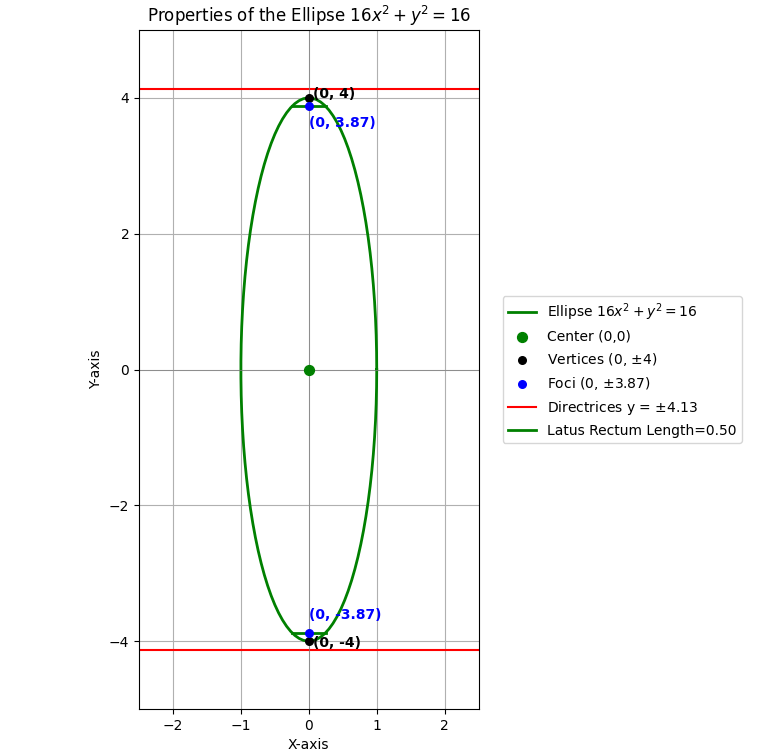
\includegraphics[width=0.7\columnwidth]{../figs/fig1.png}
\caption{}
\label{fig:1}
\end{figure}
\end{frame}

\begin{frame}{Plot by Python only}
\begin{figure}[H]
\centering
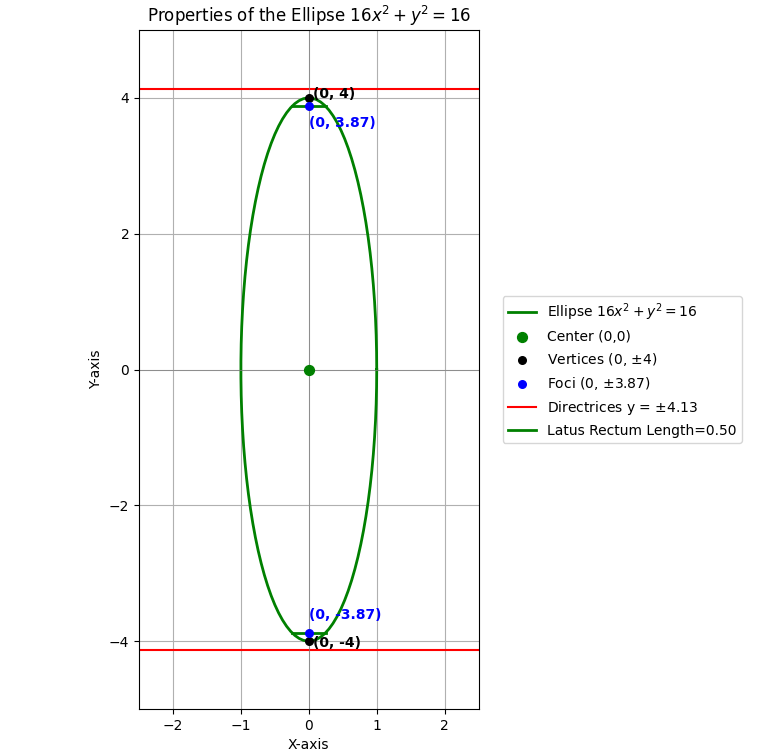
\includegraphics[width=0.7\columnwidth]{../figs/fig2.png}
\caption{}
\label{fig:2}
\end{figure}
\end{frame}

\end{document}
